\newpage
\section{\ac{SVAR} Identification} \label{SVARIdentification}
Although the model introduced in \ref{sec:MonetaryTransmissionChannels} gave us an understanding of the system, it was not derived from German economy. In this chapter we identify a model using computational tools directly from German economy.For this purpose, SVAR package in R \footcite[See.][]{Lange2020} software is used. The developed source code for this chapter is uploaded to author's Github repository.
\subsubsection{SVAR Model Identification}
The structural VAR models are often used to trace the contemporaneous linkage among macroeconomic variables. The SVAR model has the following general form  \footcite[See.][]{Lange2020}: 
\[ A_0 Y_t = \mu+  A_1(L) Y_t + B \epsilon_t \]
 Where $Y_t$ is a vector of relevant variables, then $A_0$ and $B$ are matrices and $A_1(L) = \sum\limits_{i=1}^ qA_{1i} L^i $ is the matrix polynomial in the lag operator in which $A$ matrices have the same size as $A_0$ matrix. The error terms$\epsilon_t$ (structural shocks) is a vector of serially uncorrelated zero mean structural shocks. The crucial part in \ac{SVAR} modeling is the choice of the macroeconomics variables. Besides that, the number of parameters to be identified in the structural model is larger than the reduced VAR form. Therefore, some new relations needs to be introduced. This can be usually done by introducing restrictions on $A_0$ or $B_0$ matrix. 

In this work, we introduce the following set of variables as model variables: 
The assumed $Y$ is :
\[ 
 \begin{bmatrix}
        \ac{h} \\ 
        \ac{hp} \\
        \ac{mc} \\
        \ac{rg} \\
        \ac{r} \\
        \ac{ry} \\
  \end{bmatrix}
\]

Moreover, we choose 2 as the lag number. This implies that the model takes only a history of 2 years into account.  Finally, $A_0$ is assumed to be a lower triangular matrix. The implication of this last assumption is that every variable in $Y$ vector can only be dependent on a subset of variables before it in the same year. For example \ac{hp} in year 2019 can only be function of \ac{h}  in this year and all other variables in 2018 and 2017.    


\subsection{\ac{SVAR} Results}
The Figure \ref{response} shows the impulse response of the identified model to different shocks. As one can see in Figure \ref{imp1}, when the housing supply increases housing price starts to decrease. This result matches what we expected from the monetary transmission channels. However, the plot shows a small drop in house price as a result of an increase in material cost. In my opinion, this is due to negligible affect of material cost on housing price in Germany. 
Furthermore, a close look at Figure \ref{imp2} show that after an increase in interest rate, housing price start to decrease for a period of 2 years. This result can also be explained with both IS-LM and Transition Channels model. Moreover, when housing supply increases housing price starts to decrease. Besides that, the plots imply that an increase in GDP leads to higher prices. This is also expected from an economy with growing GDP to experience and increase in house prices. However, the first plot implies that an increase in government spending can decrease the house price. In my opinion, this is not a result that one may expect. Usually an increase in government spending should lead to an increase in GDP and consequently the housing price. This impulse response can be a result of small number of lags (2 lags) chosen for the identified model and the sticky nature of housing price. Besides that, as the data set used for this identification covers only last 20 years,it can be that the data is not informative enough for this type of identification. However, this can be improved by adding feasibility constraints to the model. 
\begin{figure}[H]
\label{imp1}
\caption{Impulse Response of a Shock in Housing Supply, Housing Price and Material Cost on Housing Price}
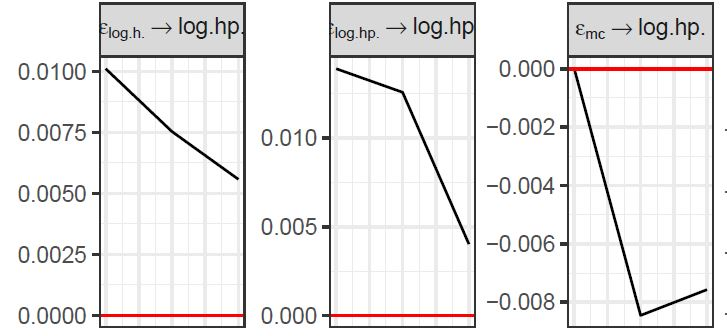
\includegraphics[width=0.9\textwidth]{hp1}
\\
Source: Own Graph
\end{figure}
\begin{figure}[H]
\label{imp2}
\caption{Impulse Response of a Shock in Government Spending, Interest Rate and Output on Housing Price}
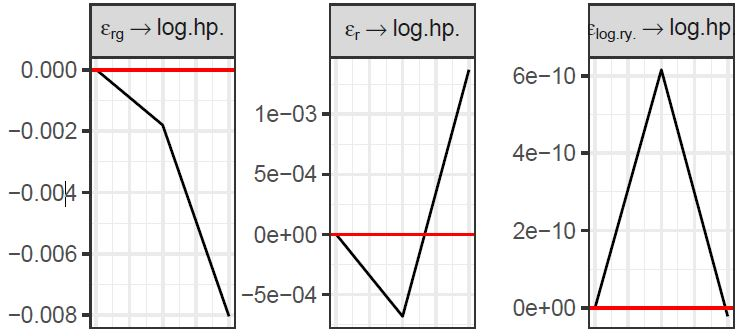
\includegraphics[width=0.9\textwidth]{hp2}
\\
Source: Own Graph
\end{figure}


